\documentclass[12pt]{article}
\usepackage[margin=1.0in]{geometry}
\usepackage{parskip}
\usepackage{graphicx}
\usepackage{caption}
\usepackage[backend=biber]{biblatex}
\usepackage[utf8]{inputenc}

\graphicspath{ {./images/} }
\addbibresource{bibliography.bib}

\begin{document}
\section{Main DSP Concepts}

We can model an analog signal as a continuous function of time $x(t)$. We can model a digital signal as a discrete sequence $\{x_n\} = \cdots, x_{-2}, x_{-1}, x_0, x_1, x_2, \cdots$, essentially a list of numbers.  With a sampling period $t_s$, we can sample an analog signal $x(n)$ to generate a digital signal $\{x_n\}$ as follows: $\{x_n\} = x(nt_s)$, or equivalently with sampling period  $f_s$, $\{x_n\} = x(\frac{n}{f_s})$

We can define discrete systems that modify a discrete sequence, and write $\{y_n\} = T\{x_n\}$ for this, where $T$ is a discrete system. We can ascribe certain properties to discrete systems; most importantly linearity and time-invariance.

If a system $T$ is linear, then it holds that $T\{x_n + y_n\} = T\{x_n\} + T\{y_n\}$

If a system $T$ is time-invariant if it holds that for any $d$, $\{y_{n-d}\} = T\{x_{n-d}\}$

Systems that have both of these properties are referred to as linear time-invariant (LTI) systems, and are of particular importance because of certain properties about them that hold. For example, the impulse response of an LTI system completely characterizes it, by convolving the an input sequence with the system's impulse response.

\subsection{The Fourier Transform}

An important operation in DSP is the Fourier transform, defined as follows on a continuous signal $x(t)$:

\[
  X(f) = \mathcal{F}\{x(t)\}(f) = \int_{-\infty}^\infty x(t)e^{-j 2 \pi f t} \mathrm{d}t
.\] 

Expanding $e^{-j2\pi f t}$, this can be rewritten as follows:
\[
  X(f) = \mathcal{F}\{x(t)\}(f) =  \int_{-\infty}^\infty x(t)\left[\cos(2\pi f t) - j\sin(2\pi f t)\right] \mathrm{d}t
.\] 

This makes the Fourier transform's purpose more obvious: we are decomposing a time signal into the frequencies of sine and cosine waves that make it up. Figure 1 shows the box function and its Fourier transform.


\begin{minipage}{\textwidth}
  \centering
  %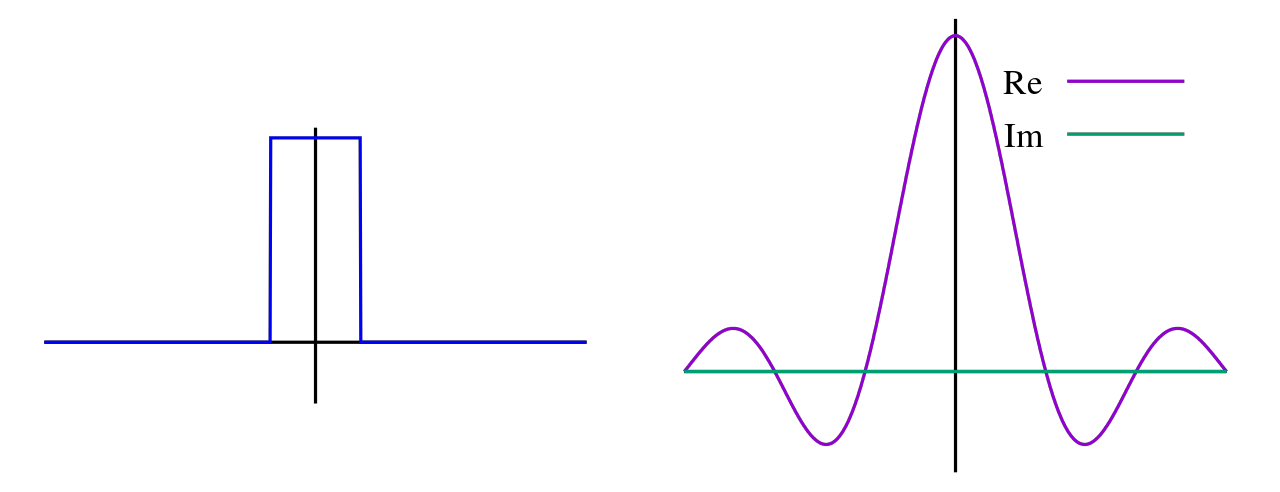
\includegraphics[trip=0 0 0, clip, scale=0.2]{fourier_transform}
  \captionof{figure}{Fourier transform of square wave}
\end{minipage}

The Fourier transform produces both real and imaginary components. If we only consider real signals, the real portion of the Fourier transform corresponds to the even parts of the signal (the cosine components), and the imaginary portion of the Fourier transform corresponds to the odd parts of the signal (the sine components). This means that the box function in Figure 1 has an entirely real Fourier transform, because it is an even function. Another property of the Fourier transform of real functions is that the the real and imaginary components will be even, so we do not gain any information from the negative parts of the transform.

The Fourier transform has some important properties. Firstly, it is linear, and furthermore there are two theorems that apply: the convolution and modulation theorem.

The convolution theorem says that convolution in the time domain is equivalent to multiplication in the frequency domain, and the modulation theorem says that multiplication in the time domain is equivalent to convolution in the frequency domain.

\subsection{The DTFT and DFT}

In digital signal processing, we work with discrete sequences, and so the traditional Fourier transform is not that useful. Instead, we use the discrete time Fourier transform (DTFT), which allows us to take the Fourier transform of a discrete sequence. It is defined as follows:

\[
  \hat{X}(f) = \mathcal{F}\{\{x_n\}\}(f) = \sum_{n=-\infty}^\infty x_n \cdot e^{-2\pi j \frac{f}{f_s}n}
\] 

This definition comes simply from taking $\{x_n\}$ as sampled from some continuous signal.

The DTFT has the same important properties of the Fourier transform as mentioned before: linearity, and adhering to the convolution and modulation theorems.

In practical use, we will be operating on finite sequences. A useful property of the Fourier transform, that holds also for the DTFT, is that if the input signal is periodic, then the resulting spectrum will be sampled, or discrete. This means that if we have some finite signal, we can turn it into an infinite discrete sequence by repeating it and making it periodic, at which point we can take the DTFT to achieve a discrete frequency spectrum. This is called the discrete Fourier transform (DFT).

To calculate it from our finite signal $x_0, \ldots, x_{N-1}$, we simply replace the bounds on the sum of our DTFT from $-\infty$ to $\infty$ with $0$ to $N-1$.

There are other discrete transforms as well. One of particular use for this project will be the discrete cosine transform (DCT) which is similar to the DFT, but transforms a discrete sequence into its representation as a sum of cosine functions, meaning that only real values are produces (unlike the DFT, which produces imaginary values as mentioned earlier). It is defined as follows on a finite sequence $x_0, \ldots x_{N-1}$:

\[
    X_k = \sum_{n=0}^{N-1} x_n\cos \left[ \frac{\pi}{N}\left(n + \frac{1}{2}\right)k\right]
\] 

\section{Quantifying Timbre}

A variety of research has been done on quantifying timbre. For example, mel frequency cepstrum coefficients (MFCCs) have been used to distinguish instruments \cite{mfcc}. Some work has also been done on quantifying timbre differences on the piano specifically \cite{pianotimbre} using partials from a power spectrum.

The MFCCs are not too hard to calculate:

\begin{itemize}
    \item
        Compute the DFT of the signal
       
    \item
        Convert the Fourier transform to the mel scale, which is intended to keep perceptually equidistant differences in pitch equidistant in the scale.

    \item
        Take the log of the spectrum

    \item
        Take the DCT of the resulting log power spectrum
\end{itemize}

In our case, we would take a short signal of a piano note onset, and calculate its MFCCs, which will be the amplitudes of the spectrum obtained in the final step of the calculation above.

It should be noted that these MFCCs will be sensitive to the pitch of notes, so some normalization might have to be done on the initial frequency spectrum to ensure fair comparison.

We can also quantify timbre using partials of a particular note. To do this, we take our power spectrum and look at the value in our Fourier transform of the integer multiples of our fundamental frequency. Of course, this requires knowing the fundamental frequency, so we will have to have some algorithms to do this, for which there exist many \cite{pitchdetectionreview}. Research suggests that higher order partials are louder in harder pressed notes than in softly pressed notes \cite{pianotimbre}.








\printbibliography


\end{document}
